\documentclass[11pt,a4paper]{article}

% ============================================================
% PACKAGES
% ============================================================

% Page layout
\usepackage[margin=1in]{geometry}
\usepackage{setspace}
\onehalfspacing

% Math
\usepackage{amsmath,amssymb,amsthm}
\usepackage{mathtools}

% Graphics and tables
\usepackage{graphicx}
\usepackage{booktabs}
\usepackage{multirow}
\usepackage{array}
\usepackage{float}
\usepackage{subcaption}

% Algorithms
\usepackage{algorithm}
\usepackage{algorithmic}

% Code listings (optional, for pseudocode)
\usepackage{listings}

% Hyperlinks and references
\usepackage[colorlinks=true,linkcolor=blue,citecolor=blue,urlcolor=blue]{hyperref}
\usepackage{cleveref}

% Bibliography
\usepackage[numbers,sort&compress]{natbib}

% Misc
\usepackage{xcolor}
\usepackage{enumitem}

% ============================================================
% CUSTOM COMMANDS
% ============================================================

% Math operators
\DeclareMathOperator*{\argmax}{arg\,max}
\DeclareMathOperator*{\argmin}{arg\,min}
\DeclareMathOperator{\E}{\mathbb{E}}

% Vectors and matrices
\newcommand{\vect}[1]{\mathbf{#1}}
\newcommand{\mat}[1]{\mathbf{#1}}

% Common symbols
\newcommand{\R}{\mathbb{R}}
\newcommand{\N}{\mathbb{N}}

% State, action, reward
\newcommand{\state}{\vect{s}}
\newcommand{\action}{\vect{a}}
\newcommand{\reward}{r}

% ============================================================
% DOCUMENT INFO
% ============================================================

\title{Deep Reinforcement Learning for Cryptocurrency Portfolio Management: \\
A Comparative Study}

\author{
Jose Luis Marquez Jaramillo, Taylor Hawks \\
EN.605.741 - Reinforcement Learning\\
Johns Hopkins University 
}

\date{December 2025}

% ============================================================
% DOCUMENT
% ============================================================

\begin{document}

\maketitle

% ------------------------------------------------------------
% ABSTRACT
% ------------------------------------------------------------
% ============================================================
% ABSTRACT
% ============================================================

\begin{abstract}

% BACKGROUND: What is the problem?
Cryptocurrency markets present unique challenges for portfolio management due to their high volatility, 24/7 trading, and evolving asset universe.

% OBJECTIVE: What did you do?
We investigate the application of deep reinforcement learning (DRL) to dynamic cryptocurrency portfolio allocation, implementing and comparing three RL agents---Deep Q-Network (DQN), Double DQN (DDQN), and REINFORCE---against traditional baselines including Equal Weight, Market Cap Weight, and Mean-Variance Optimization.

% METHODS: How did you do it?
Our environment processes over seven years of historical data (2018--2025) for 37 cryptocurrencies, using a 60-day lookback window of OHLCV features. We design a discrete action space with 70 delta-based portfolio adjustments for value-based methods and a continuous simplex output for policy gradient methods, incorporating realistic constraints including transaction costs (0.1\%) and turnover limits (30\%).

% RESULTS: What did you find?
On a held-out test period (January 2024--October 2025), the Mean-Variance baseline achieved the highest cumulative return (366.54\%) and Sharpe ratio (1.64), followed by Equal Weight (168.50\%, Sharpe 1.22). Among RL agents, REINFORCE performed best (166.98\%, Sharpe 1.21), with DQN (155.47\%) and DDQN (144.50\%) trailing behind.

% CONCLUSIONS: What does it mean?
Our results suggest that in the tested market regime, classical optimization methods outperformed learned policies, highlighting challenges in sample efficiency and generalization for DRL in financial applications. We discuss implications for future research directions.

\end{abstract}


% ------------------------------------------------------------
% MAIN SECTIONS
% ------------------------------------------------------------
% ============================================================
% INTRODUCTION
% ============================================================

\section{Introduction}
\label{sec:introduction}

% HOOK: Why should the reader care? - Now with quantitative, cited facts
The cryptocurrency market has grown from a niche experiment to a multi-trillion-dollar asset class, with total market capitalization exceeding \$3.20 trillion as of December 2025 \cite{forbes2025crypto}, surpassing the previous peak of approximately \$3 trillion in November 2021 \cite{pessa2023age, watorek2023crypto}. This growth brings unique challenges for portfolio management: daily volatility that frequently exceeds traditional equity markets by several times \cite{bergsli2022volatility, naimy2021garch}, continuous 24/7 trading across fragmented exchanges with varying transaction costs \cite{barbon2021exchanges, kim2017transaction}, and an evolving asset universe as new tokens emerge and others fail. Furthermore, cross-asset correlations in cryptocurrency markets shift substantially between bull and bear regimes \cite{james2022correlations}, complicating covariance estimation for traditional optimization approaches.

% CONTEXT: Background on the problem
Deep reinforcement learning (DRL) has demonstrated strong performance in sequential decision-making domains from game playing to robotics, prompting researchers to explore its application to financial portfolio management \cite{jiang2017eIIE, lucarelli2020dqlcrypto}. The portfolio management problem---dynamically allocating capital across multiple assets to maximize risk-adjusted returns---naturally maps to a Markov Decision Process (MDP). At each decision point, the agent observes market conditions and its current holdings, then selects target portfolio weights subject to constraints such as position limits and transaction costs. Unlike supervised learning approaches that predict returns and then optimize, RL directly learns the allocation policy end-to-end, potentially capturing complex temporal dependencies and trading off immediate costs against future opportunities.

% GAP: What's missing in current approaches?
Despite promising results in controlled experiments, applying DRL to real-world portfolio management faces several challenges that prior work has incompletely addressed. First, most studies assume a fixed asset universe \cite{jiang2017eIIE, ye2020sarl}, but cryptocurrency portfolios must handle assets entering and leaving the tradable set as market conditions change. Second, the choice of action space---whether continuous weights, discrete allocation templates, or incremental adjustments---significantly affects learning dynamics but remains underexplored \cite{lucarelli2020dqlcrypto}. Third, rigorous comparison against strong traditional baselines is often lacking; the equal-weight (1/N) portfolio, despite its simplicity, has proven remarkably difficult to beat in out-of-sample tests \cite{demiguel2009optimal}.

% OBJECTIVE: What does this paper do?
This paper investigates whether deep reinforcement learning can learn profitable portfolio allocation strategies for cryptocurrency markets that outperform classical approaches. We develop a comprehensive experimental framework that addresses the practical challenges of variable asset universes, realistic transaction costs, and fair comparison across different algorithmic paradigms. Our goal is not merely to achieve positive returns---which depend heavily on the test period---but to understand under what conditions and architectural choices DRL methods succeed or fail relative to traditional baselines.

% APPROACH: How do we address it?
Our approach combines a realistic portfolio environment with multiple agent architectures. The environment handles monthly universe reconstitution, enforces trading constraints (turnover limits, concentration caps), and applies proportional transaction costs consistent with centralized exchange fee structures \cite{brauneis2022fees}. We implement four DRL agents spanning value-based and policy gradient paradigms: Deep Q-Network (DQN) with a novel delta-based action catalog, Double DQN (DDQN) to address overestimation bias \cite{vanHasselt2016ddqn}, REINFORCE for continuous policy optimization \cite{williams1992reinforce}, and REINFORCE with a learned value baseline to reduce gradient variance. These are benchmarked against three traditional strategies: equal weighting, market-capitalization weighting, and mean-variance optimization with shrinkage estimation \cite{ledoit2004honey}.

% CONTRIBUTIONS: What are the key contributions? - Consolidated from 5 to 4, merged reproducibility into first contribution
\paragraph{Contributions.} The main contributions of this work are:
\begin{enumerate}[leftmargin=*]
    \item \textbf{Variable universe environment}: A portfolio management environment handling dynamic asset membership with monthly reconstitution, cold-start rules, and automatic weight redistribution. We release a frozen dataset export enabling exact reproduction.
    
    \item \textbf{Delta-based discrete action space}: A 70-action catalog of relative portfolio adjustments for DQN agents, preserving portfolio continuity and enabling context-dependent feasibility learning.
    
    \item \textbf{Canonical padding for variable-size observations}: A scheme mapping variable-size observations to fixed-dimensional representations while preserving asset identity for Q-value learning.
    
    \item \textbf{Rigorous out-of-sample evaluation}: A 646-day held-out test demonstrating that DDQN outperforms passive baselines, and that policy gradient methods achieve competitive performance under deterministic evaluation.
\end{enumerate}

% OUTLINE: Paper structure
\paragraph{Paper organization.} The remainder of this paper is organized as follows. \Cref{sec:related_work} reviews related work in deep reinforcement learning for portfolio management and positions our contributions. \Cref{sec:methods} describes our environment design, agent architectures, and baseline implementations in detail. \Cref{sec:experiments} presents the experimental setup, training procedures, and quantitative results. \Cref{sec:discussion} interprets the divergent outcomes between value-based and policy gradient methods and discusses limitations. \Cref{sec:conclusion} concludes with directions for future research.

% ============================================================
% RELATED WORK
% ============================================================

\section{Related Work}
\label{sec:related_work}

We review prior work in four areas: deep reinforcement learning for portfolio management, value-based and policy gradient methods, traditional portfolio optimization, and the unique characteristics of cryptocurrency markets that motivate our design choices.

% ------------------------------------------------------------
\subsection{Deep Reinforcement Learning for Portfolio Management}
\label{subsec:drl_portfolio}
% ------------------------------------------------------------

The application of deep reinforcement learning to portfolio management was pioneered by \citet{jiang2016drlt}, who introduced the Ensemble of Identical Independent Evaluators (EIIE) framework for cryptocurrency trading. This architecture processes each asset's price history through identical neural network modules, producing allocation scores that are normalized via softmax to obtain portfolio weights. The follow-up work \cite{jiang2017eIIE} extended this framework with the Portfolio Vector Memory (PVM), which feeds the previous portfolio weights back into the policy network. This recurrent structure helps the agent internalize transaction costs by learning to avoid unnecessary rebalancing.

\citet{ye2020sarl} proposed State-Augmented Reinforcement Learning (SARL), which enriches the observation space with market-wide indicators such as index returns and volatility measures. By conditioning on broader market context, SARL agents can potentially adapt their strategies to different market regimes. The authors demonstrated improved performance on Chinese stock markets compared to baseline methods.

\citet{lucarelli2020dqlcrypto} applied Deep Q-Learning to cryptocurrency trading, exploring discrete action spaces where each action corresponds to a complete portfolio allocation. Their work highlighted the challenges of applying DQN to portfolio management, including the need for careful reward shaping and the difficulty of learning in highly non-stationary financial environments.

\paragraph{Limitations of prior DRL approaches.} Despite promising backtested results, several limitations persist across this literature. First, most studies assume a fixed asset universe throughout training and evaluation, which does not reflect the reality of cryptocurrency markets where tokens are frequently listed and delisted. Second, evaluation periods are often short or overlap with training data, making it difficult to assess true generalization. Third, comparison against traditional baselines is frequently limited to buy-and-hold strategies, which can underperform in trending markets and provide limited insight into whether DRL adds value over established portfolio optimization methods. Our work addresses these gaps by explicitly modeling variable universes, using strict train/test separation, and benchmarking against strong traditional methods.

% ------------------------------------------------------------
\subsection{Value-Based and Policy Gradient Methods}
\label{subsec:rl_methods}
% ------------------------------------------------------------

Deep Q-Networks (DQN)~\citep{mnih2015dqn} combine Q-learning with neural networks and experience replay, but suffer from overestimation bias. Double DQN~\citep{vanHasselt2016ddqn} addresses this by decoupling action selection from evaluation. Applying DQN to portfolio management requires discretizing the action space; \citet{gao2020dqnportfolio} used fixed allocation templates, but this scales poorly with universe size. Our delta-based action catalog defines actions as relative portfolio changes, enabling smooth transitions through portfolio space.

REINFORCE~\citep{williams1992reinforce} naturally handles continuous action spaces and has been applied to portfolio management where weights are treated as continuous outputs. Actor-critic methods reduce variance through learned baselines~\citep{sutton1999policy, sadighian2019mmppo}. The EIIE framework~\citep{jiang2017eIIE} uses softmax outputs to satisfy simplex constraints; our REINFORCE implementation follows this paradigm with Dirichlet sampling for exploration.

% ------------------------------------------------------------
\subsection{Traditional Portfolio Optimization}
\label{subsec:traditional}
% ------------------------------------------------------------

Mean-variance optimization, introduced by \citet{markowitz1952portfolio}, remains the foundation of quantitative portfolio management. The framework selects portfolio weights to maximize expected return for a given level of variance, or equivalently, minimize variance for a target return. However, mean-variance optimization is highly sensitive to estimation error in expected returns and covariances.

\citet{demiguel2009optimal} compared fourteen portfolio strategies across multiple datasets, finding that the simple equal-weight (1/N) portfolio frequently outperformed optimized strategies out-of-sample. Their analysis attributed this to estimation error: the benefits of optimization are overwhelmed by the noise in estimated parameters, particularly expected returns. This result established equal weighting as a baseline that optimized strategies often fail to beat.

To improve robustness, practitioners employ shrinkage estimators for covariance matrices. \citet{ledoit2004honey} proposed shrinking the sample covariance toward a structured target (e.g., diagonal or constant correlation), reducing estimation error at the cost of some bias. Our mean-variance baseline implements Ledoit-Wolf shrinkage, representing a reasonable best-effort classical approach.

\paragraph{Challenges for traditional methods in cryptocurrency markets.} While mean-variance optimization has been extensively studied for equity portfolios, cryptocurrency markets present additional challenges. Return distributions exhibit heavy tails and time-varying volatility that violate the Gaussian assumptions underlying mean-variance theory \cite{bergsli2022volatility, naimy2021garch}. Cross-asset correlations shift substantially between bull and bear market regimes \cite{james2022correlations}, meaning covariance estimates from calm periods may be misleading during crises. Furthermore, the short history of most cryptocurrencies limits the statistical reliability of parameter estimates. These characteristics motivate exploring whether data-driven RL methods can learn more adaptive allocation strategies.

% ------------------------------------------------------------
\subsection{Positioning of This Work}
\label{subsec:positioning}
% ------------------------------------------------------------

Our work extends prior DRL portfolio research by addressing three key gaps. First, unlike EIIE \cite{jiang2017eIIE} and SARL \cite{ye2020sarl}, we explicitly model variable asset universes with monthly reconstitution and eligibility rules. Second, our delta-based action catalog enables smooth portfolio transitions while maintaining a tractable discrete action space for value-based learning. Third, our canonical padding state encoder preserves asset identity information essential for evaluating delta actions.

We contribute to the broader discussion about the practical value of DRL for portfolio management. While prior work has often reported positive results in backtesting, rigorous out-of-sample evaluation has been limited. Our 646-day test period reveals that both algorithmic paradigm and inference-time behavior matter: value-based methods with discrete actions outperform passive baselines, while continuous policy gradient methods achieve competitive performance when using deterministic evaluation (outputting the distribution mean rather than sampling). These findings suggest that action space design and deployment strategy deserve more systematic attention than they have received in prior work.

% ============================================================
% METHODS
% ============================================================

\section{Methods}
\label{sec:methods}

This section describes our methodology for applying deep reinforcement learning to cryptocurrency portfolio management. We first formalize the problem as a Markov Decision Process (\Cref{sec:problem_formulation}), then detail our environment design including data processing and constraint handling (\Cref{sec:environment}). We present four RL agent architectures (\Cref{sec:agents}) and three baseline strategies (\Cref{sec:baselines}) that operate under identical constraints for fair comparison.

% ------------------------------------------------------------
\subsection{Problem Formulation}
\label{sec:problem_formulation}
% ------------------------------------------------------------

We formulate cryptocurrency portfolio management as a Markov Decision Process (MDP) defined by the tuple $(\mathcal{S}, \mathcal{A}, \mathcal{P}, \mathcal{R}, \gamma)$, where $\mathcal{S}$ is the state space, $\mathcal{A}$ is the action space, $\mathcal{P}$ defines transition dynamics, $\mathcal{R}$ is the reward function, and $\gamma \in [0,1]$ is the discount factor.

\paragraph{Transition Dynamics.} The transition $\mathcal{P}(s_{t+1}|s_t, a_t)$ is determined by two components: (1) exogenous market price movements, which we do not model or predict, and (2) endogenous portfolio mechanics, where the new weights $\vect{w}_t$ become the ``previous weights'' in the next state. We adopt a model-free approach---agents learn directly from environment interactions without estimating $\mathcal{P}$.

\paragraph{State Space.} At each trading day $t$, the state $s_t$ consists of (1) a per-asset historical observation tensor $\mat{X}_t \in \R^{A_t \times 4 \times 60}$ containing normalized OHLCV features over a 60-day lookback window, and (2) the previous portfolio weights $\vect{w}_{t-1} \in \Delta^{A_{t-1}}$, where $A_t$ denotes the number of tradable assets at time $t$. The inclusion of previous weights, analogous to the Portfolio Vector Memory (PVM) mechanism~\citep{jiang2017eIIE}, enables the agent to internalize turnover costs.

\paragraph{Action Space.} The action $a_t$ specifies a target portfolio allocation $\vect{w}_t \in \Delta^{A_t}$ over the current tradable assets. For value-based methods, we discretize this space into 70 delta-based rebalancing actions (\Cref{sec:dqn}); for policy gradient methods, we output continuous weights directly (\Cref{sec:reinforce}).

\paragraph{Constraints.} All portfolios must satisfy:
\begin{align}
    w_t^{(i)} &\geq 0 \quad \forall i \quad \text{(long-only)} \label{eq:long_only} \\
    \sum_{i=1}^{A_t} w_t^{(i)} &= 1 \quad \text{(fully invested, no cash)} \label{eq:simplex} \\
    \|\vect{w}_t - \vect{w}_{t-1}\|_1 &\leq \tau \quad \text{(turnover limit, } \tau = 0.30\text{)} \label{eq:turnover}
\end{align}

The fully-invested constraint~\eqref{eq:simplex} forces the agent to maintain exposure to cryptocurrency risk rather than trivially holding cash, ensuring fair comparison against crypto benchmarks~\citep{jiang2017eIIE, lucarelli2020dqlcrypto}.

\paragraph{Reward Function.} The agent receives a reward based on net portfolio return after transaction costs:
\begin{equation}
    r_t = \log\left(1 + \vect{w}_t^\top \vect{R}_{t+1}\right) - c \cdot \|\vect{w}_t - \vect{w}_{t-1}\|_1
    \label{eq:reward}
\end{equation}
where $\vect{R}_{t+1} \in \R^{A_t}$ is the vector of simple returns from day $t$ to $t+1$, and $c = 0.001$ is the transaction cost coefficient (0.1\% per unit turnover). Critically, the forward returns $\vect{R}_{t+1}$ are never observed by the agent at decision time---they are used only by the environment to compute realized rewards after the action is taken.

\paragraph{Objective.} The agent seeks to maximize expected cumulative discounted rewards:
\begin{equation}
    \max_\pi \; \E_\pi \left[ \sum_{t=0}^{T} \gamma^t r_t \right]
\end{equation}
We use $\gamma = 0.93$ for production training, selected via Bayesian hyperparameter optimization (\Cref{sec:hyperparameters}). This relatively high discount factor indicates that longer-horizon planning is beneficial even with daily transaction costs, though the search space included values as low as 0.5.

% ------------------------------------------------------------
\subsection{Environment Design}
\label{sec:environment}
% ------------------------------------------------------------

Our environment processes over seven years of cryptocurrency market data and enforces realistic trading constraints. We describe the data pipeline, state representation, and constraint enforcement mechanisms.

\subsubsection{Data Pipeline}

We use daily OHLCV (Open, High, Low, Close, Volume) data for liquid cryptocurrencies from 2018-07-01 through 2025-10-31. The tradable universe is defined by a market-cap-weighted index with monthly constituent rebalancing: at the end of month $m-1$, we freeze the index membership for all days in month $m$, preventing intramonth look-ahead bias.

\paragraph{Data Quality.} We apply tiered gap repair rules to handle missing data. Single-day gaps are addressed through forward-filling, propagating the previous day's bar. Gaps of two to five days receive linear interpolation for price channels and log-space interpolation for volume to preserve multiplicative scaling properties. Gaps exceeding five days trigger asset ineligibility---the asset is excluded from the tradable universe until 60 consecutive days of clean data become available, ensuring sufficient history for feature construction.

\paragraph{Cold-Start Eligibility.} An asset is tradable on day $t$ only if it (1) is included in the current month's index membership, and (2) has at least 60 consecutive days of clean OHLCV data immediately prior to $t$. This prevents allocation to newly listed or illiquid assets with insufficient trading history~\citep{jiang2017eIIE, ye2020sarl}.

\subsubsection{State Representation}

For each tradable asset $i$ at time $t$, we construct a feature tensor from the trailing 60-day window:

\paragraph{Price Normalization.} Close, high, and low prices are divided by the asset's closing price on day $t$, so the most recent close equals 1.0 and prior prices are relative. This improves stationarity and has been shown to stabilize training in crypto portfolio agents~\citep{jiang2017eIIE}.

\paragraph{Volume Normalization.} We apply $\log(1 + \text{volume})$, then z-score normalize within each asset's 60-day window, clipping extreme values to $[-5, 5]$.

The resulting observation tensor $\mat{X}_t \in \R^{A_t \times 4 \times 60}$ has dimensions: $A_t$ assets $\times$ 4 channels (close, high, low, volume) $\times$ 60 days. Because $A_t$ varies over time (due to index rebalancing and cold-start rules), we employ canonical padding for value-based methods (\Cref{sec:dqn}).

\paragraph{Universe Changes.} When assets exit the tradable universe (due to index rebalancing or data quality issues), the environment forces liquidation at the last available price and redistributes the weight proportionally across remaining assets, incurring transaction costs. New entrants begin with zero weight and become available for allocation only after satisfying the cold-start requirement.

\subsubsection{Constraint Enforcement}
\label{sec:constraint_enforcement}

The environment supports two constraint handling approaches:

\paragraph{Projection Mode} (used by REINFORCE): If the proposed allocation violates constraints, the environment projects it onto the feasible set using quadratic programming. The agent is trained on the projected allocation without explicit feedback about violations.

\paragraph{Penalty Mode} (used by DQN/DDQN): If the proposed allocation violates constraints, the environment rejects execution and assigns a penalty reward of $-10.0$. The portfolio remains at its previous state, but time advances normally. The penalty magnitude was chosen to be substantially larger than typical single-step rewards (which range from approximately $-0.05$ to $+0.05$), ensuring constraint violations are strongly discouraged. This enables the agent to learn context-dependent feasibility through experience---the same delta action (e.g., ``increase BTC by 10\%'') can be safe or risky depending on current holdings~\citep{lucarelli2020dqlcrypto}.

% ------------------------------------------------------------
\subsection{Agent Architectures}
\label{sec:agents}
% ------------------------------------------------------------

We implement two reinforcement learning agent families: value-based methods (DQN, DDQN) and policy gradient methods (REINFORCE, REINFORCE with learned baseline).

% ----------------------------
\subsubsection{Deep Q-Network (DQN) and Double DQN (DDQN)}
\label{sec:dqn}
% ----------------------------

Our value-based agents address two key challenges: handling variable universe sizes with fixed-dimensional networks, and designing a discrete action space for portfolio rebalancing.

\paragraph{Canonical Padding StateEncoder.}
We assign each of the 37 unique assets a fixed canonical position. For each observation, we populate zero-padded arrays $\mat{X}_{\text{canonical}} \in \R^{37 \times 4 \times 60}$ and $\vect{w}_{\text{canonical}} \in \R^{37}$ at assigned positions, then flatten to 8,917 dimensions and project through a learned linear layer to a 256-dimensional embedding. This preserves asset identity essential for context-dependent Q-values.

\paragraph{Delta-Based Action Catalog.}
We implement 70 discrete portfolio adjustment actions: a hold action; adjust actions that increase/decrease exposure to top-$K$ assets by $\pm5\%$, $\pm10\%$, or $\pm15\%$; rotation actions transferring weight between asset pairs; and rebalancing actions resetting to equal weight or market-cap weight. Each action applies a delta adjustment and renormalizes to the simplex.

\paragraph{Network Architecture and Training.}
The Q-network is a 3-layer MLP (512$\rightarrow$256$\rightarrow$70) with ReLU and dropout. We use experience replay (capacity 10,000), $\epsilon$-greedy exploration decaying from 1.0 to 0.1, and target network updates every 100 steps. DDQN differs only in the TD target: $Q_{\text{target}} = r + \gamma \, Q_{\text{target}}(s', \argmax_{a'} Q_{\text{online}}(s', a'))$, decoupling action selection from evaluation to reduce overestimation bias~\citep{vanHasselt2016ddqn}.

% ----------------------------
\subsubsection{REINFORCE Policy Gradient Agents} 
\label{sec:reinforce} 
% ---------------------------- 
Our policy gradient agents directly parameterize portfolio weights as continuous outputs. \paragraph{Policy Network Architecture.} A GRU layer (input size $4 \times N$, sequence length=60) processes the combined assets' 60-day sequence.  The GRU layer outputs to a fully connected layer where it is concatenated with the previous weights and a binary initialization flag.  This is then fed to another hidden layer then to a final output layer which produces per-asset logits, converted via masked softmax to portfolio weights. We use canonical indexing across 37 positions with a boolean mask for tradable assets. 
 
\paragraph{Training with Dirichlet Sampling.} Actions are sampled from a Dirichlet distribution with concentration parameters $\boldsymbol{\alpha} = \text{softplus}(\text{logits}) / \tau$, where temperature $\tau$ is a parameter introduced to flatten or spike the distribution. When sampled allocations violate constraints, the environment projects them onto the feasible set. Policy gradients use Monte Carlo returns, and the network uses an Adam optimizer.
 
\paragraph{Learned Value Baseline.} To reduce gradient variance, REINFORCE+Baseline adds a value head $V_\phi(s_t)$, which shares the GRU encoder for learning efficiency. The advantage $A_t = G_t - V_\phi(s_t)$ replaces raw returns in the policy gradient. The combined loss is $\mathcal{L} = -\sum_t A_t \log \pi_\theta(a_t | s_t) + 0.5 \sum_t (G_t - V_\phi(s_t))^2$.
 
% ------------------------------------------------------------
\subsection{Baselines}
\label{sec:baselines}
% ------------------------------------------------------------

We implement three baselines operating under identical constraints. \textbf{Equal Weight (EW)} allocates uniformly: $w_t^{(i)} = 1/A_t$. Despite its simplicity, equal weighting has proven competitive by avoiding estimation error~\citep{demiguel2009optimal}. \textbf{Market Cap Weight (MCW)} allocates proportionally to market capitalization, mimicking index funds with minimal turnover. \textbf{Mean-Variance Optimization (MVO)} implements Markowitz optimization~\citep{markowitz1952portfolio}:
\begin{equation}
    \vect{w}_t^* = \argmax_{\vect{w} \in \Delta^{A_t}} \left\{ \vect{w}^\top \hat{\boldsymbol{\mu}}_t - \frac{\lambda}{2} \vect{w}^\top \hat{\boldsymbol{\Sigma}}_t \vect{w} \right\}
\end{equation}
using Ledoit-Wolf shrinkage~\citep{ledoit2004honey} for covariance estimation.

% ============================================================
% EXPERIMENTS
% ============================================================

\section{Experiments}
\label{sec:experiments}

This section describes our experimental setup and presents the results of our comparative evaluation. We detail the dataset construction (\Cref{sec:dataset}), evaluation metrics (\Cref{sec:metrics}), hyperparameter selection process (\Cref{sec:hyperparameters}), and present the main results (\Cref{sec:results}).

% ------------------------------------------------------------
\subsection{Dataset}
\label{sec:dataset}
% ------------------------------------------------------------

We construct a comprehensive cryptocurrency dataset spanning over seven years of market data.

\paragraph{Data Source.} Daily OHLCV (Open, High, Low, Close, Volume) data is collected from Binance via the CCXT library. The dataset covers 37 unique cryptocurrencies, with daily availability varying between 8 and 35 assets depending on index membership and cold-start eligibility requirements.

\paragraph{Temporal Splits.} We partition the data into non-overlapping periods following walk-forward evaluation principles~\citep{lucarelli2020dqlcrypto}:

\begin{table}[htbp]
\centering
\caption{Dataset temporal splits. The warmup period builds initial lookback windows. Development data is used for training and hyperparameter selection. Test data is strictly held out for final evaluation.}
\label{tab:splits}
\begin{tabular}{llrl}
\toprule
\textbf{Split} & \textbf{Period} & \textbf{Days} & \textbf{Purpose} \\
\midrule
Warmup & 2018-07-01 $\rightarrow$ 2018-08-31 & 62 & Build 60-day lookback \\
Train (train\_core) & 2018-09-01 $\rightarrow$ 2023-06-30 & 1,848 & Agent training \\
Validation & 5 regime windows & ${\sim}$100 & Hyperparameter selection \\
Test & 2024-01-01 $\rightarrow$ 2025-10-31 & 646 & Out-of-sample evaluation \\
\bottomrule
\end{tabular}
\end{table}

\paragraph{Regime-Based Validation.} Rather than using a single contiguous validation period, we carve out five approximately 20-day windows corresponding to qualitatively distinct market regimes. These include the late 2018 cryptocurrency winter (val\_2018\_crash), the March 2020 COVID-induced market crash (val\_covid), the 2021 bull market (val\_bull), the 2022 deleveraging period (val\_bear), and the 2023 low-volatility consolidation (val\_chop). This regime-diverse validation strategy prevents overfitting hyperparameters to a single market condition~\citep{jiang2016drlt, jiang2017eIIE}, ensuring that selected configurations generalize across bull markets, bear markets, and high-volatility crash periods alike.

% ------------------------------------------------------------
\subsection{Evaluation Metrics}
\label{sec:metrics}
% ------------------------------------------------------------

We evaluate portfolio performance using standard metrics from quantitative finance, encompassing return measures, risk metrics, and trading activity indicators.

\paragraph{Return Metrics.} Cumulative return measures the total percentage gain over the evaluation period, providing an absolute performance benchmark. We also report the Compound Annual Growth Rate (CAGR), which annualizes returns while properly accounting for compounding effects, enabling comparison across periods of different lengths.

\paragraph{Risk-Adjusted Performance.} The Sharpe ratio~\citep{sharpe1966mutual} quantifies risk-adjusted return as the ratio of annualized excess return to annualized volatility, assuming a zero risk-free rate given the cryptocurrency context. We complement this with the Sortino ratio, which penalizes only downside volatility by using only negative returns in the denominator, providing a measure more aligned with investor preferences. Maximum drawdown captures the largest peak-to-trough decline observed during the evaluation period, representing worst-case loss exposure. The Calmar ratio, computed as CAGR divided by maximum drawdown, combines these perspectives into a single efficiency metric.

\paragraph{Trading Activity.} Portfolio turnover, defined as the mean daily $L_1$ norm of weight changes $\|\vect{w}_t - \vect{w}_{t-1}\|_1$, quantifies trading activity. High turnover strategies incur greater transaction costs, making this metric essential for assessing practical viability in markets with non-trivial trading frictions.

% ------------------------------------------------------------
\subsection{Hyperparameter Selection}
\label{sec:hyperparameters}
% ------------------------------------------------------------

We employ Bayesian hyperparameter optimization using Optuna~\citep{optuna2019} to efficiently search the high-dimensional configuration space.

\paragraph{Search Protocol.} For the value-based DQN and DDQN agents, we use the Tree-structured Parzen Estimator (TPE) sampler to guide the search over 50 candidate configurations. Each configuration is evaluated by training for 50 episodes using 100-day sliding windows sampled from the training period, followed by validation across five episodes on the regime-diverse validation windows with a fixed random seed for reproducibility. The optimization objective maximizes mean validation return, with MedianPruner providing early termination for unpromising trials. We additionally implement Q-value explosion detection, terminating any trial where mean Q-values exceed 10,000 to prevent numerical instability from wasting computational resources.

\paragraph{Search Space.} The hyperparameter ranges explored are shown in \Cref{tab:search_space}. The discount factor $\gamma$ spans from 0.5 to 0.99, accommodating both short-horizon and long-horizon reward weighting. Learning rates are sampled log-uniformly between $10^{-5}$ and $10^{-3}$ to cover several orders of magnitude. Architectural choices include batch sizes of 32, 64, or 128, replay buffer capacities of 10,000 or 50,000 transitions, and network hidden dimensions ranging from two-layer configurations ([128, 64]) to deeper three-layer architectures ([512, 256, 128]). Exploration parameters include $\epsilon$ decay schedules of 300, 500, or 1,000 episodes and terminal $\epsilon$ values between 0.01 and 0.1.

\begin{table}[htbp]
\centering
\caption{Hyperparameter search space for DQN/DDQN agents.}
\label{tab:search_space}
\begin{tabular}{lll}
\toprule
\textbf{Hyperparameter} & \textbf{Range} & \textbf{Scale} \\
\midrule
Discount factor ($\gamma$) & $[0.5, 0.99]$ & Uniform \\
Learning rate & $[10^{-5}, 10^{-3}]$ & Log-uniform \\
Batch size & $\{32, 64, 128\}$ & Categorical \\
Replay buffer size & $\{10{,}000, 50{,}000\}$ & Categorical \\
$\epsilon$ decay episodes & $\{300, 500, 1000\}$ & Categorical \\
$\epsilon$ final & $[0.01, 0.1]$ & Uniform \\
Target update frequency & $\{50, 100, 200\}$ & Categorical \\
Hidden dimensions & $\{[128,64], [256,128], [512,256,128]\}$ & Categorical \\
\bottomrule
\end{tabular}
\end{table}

\paragraph{Training Protocol.} Using the best hyperparameters identified through the search, we train the final models with extended episode budgets. DQN trains for 400 episodes and DDQN for 300 episodes, both using 100-day sliding windows sampled from the training period. The REINFORCE agent, contributed as a separate implementation with independent tuning, trains for 10,000 episodes. All agents employ early stopping with patience of 5 validation checks (performed every 50 episodes for value-based methods) to prevent overfitting, and we checkpoint the best model based on mean validation return for final evaluation.

% ------------------------------------------------------------
\subsection{Results}
\label{sec:results}
% ------------------------------------------------------------

We evaluate all six strategies on the held-out test period (January 2024 -- October 2025, 646 trading days). Results are summarized in \Cref{tab:main_results} and visualized in Figures~\ref{fig:cumulative_returns}--\ref{fig:allocation_comparison}.

% Main results table
\begin{table}[htbp]
\centering
\caption{Test set performance comparison across all agents and baselines. Best values in \textbf{bold}, second-best \underline{underlined}. Test period: January 2024 -- October 2025 (646 trading days).}
\label{tab:main_results}
\begin{tabular}{lcccccc}
\toprule
\textbf{Agent} & \textbf{Return (\%)}  & \textbf{CAGR (\%)} & \textbf{Sharpe} & \textbf{Sortino} & \textbf{Max DD (\%)} & \textbf{Turnover (\%)} \\
\midrule
\multicolumn{7}{l}{\textit{Baselines}} \\
Equal Weight     & \underline{168.50} & \underline{74.88} & 1.217 & 1.250 & 48.87 & \textbf{0.25} \\
Market Cap       & 159.30 & 71.46 & \underline{1.240} & \underline{1.298} & \underline{44.17} & 0.34 \\
Mean-Variance    & \textbf{366.54} & \textbf{139.07} & \textbf{1.640} & \textbf{1.691} & \textbf{39.96} & 13.50 \\
\midrule
\multicolumn{7}{l}{\textit{RL Agents}} \\
DQN              & 155.47 & 70.03 & 1.146 & 1.175 & 52.59 & 10.88 \\
DDQN             & 144.50 & 65.85 & 1.135 & 1.157 & 52.56 & 8.39 \\
REINFORCE        & 166.98 & 74.32 & 1.212 & 1.247 & 48.72 & 0.82 \\
\bottomrule
\end{tabular}
\end{table}

% Cumulative returns figure
\begin{figure}[htbp]
    \centering
    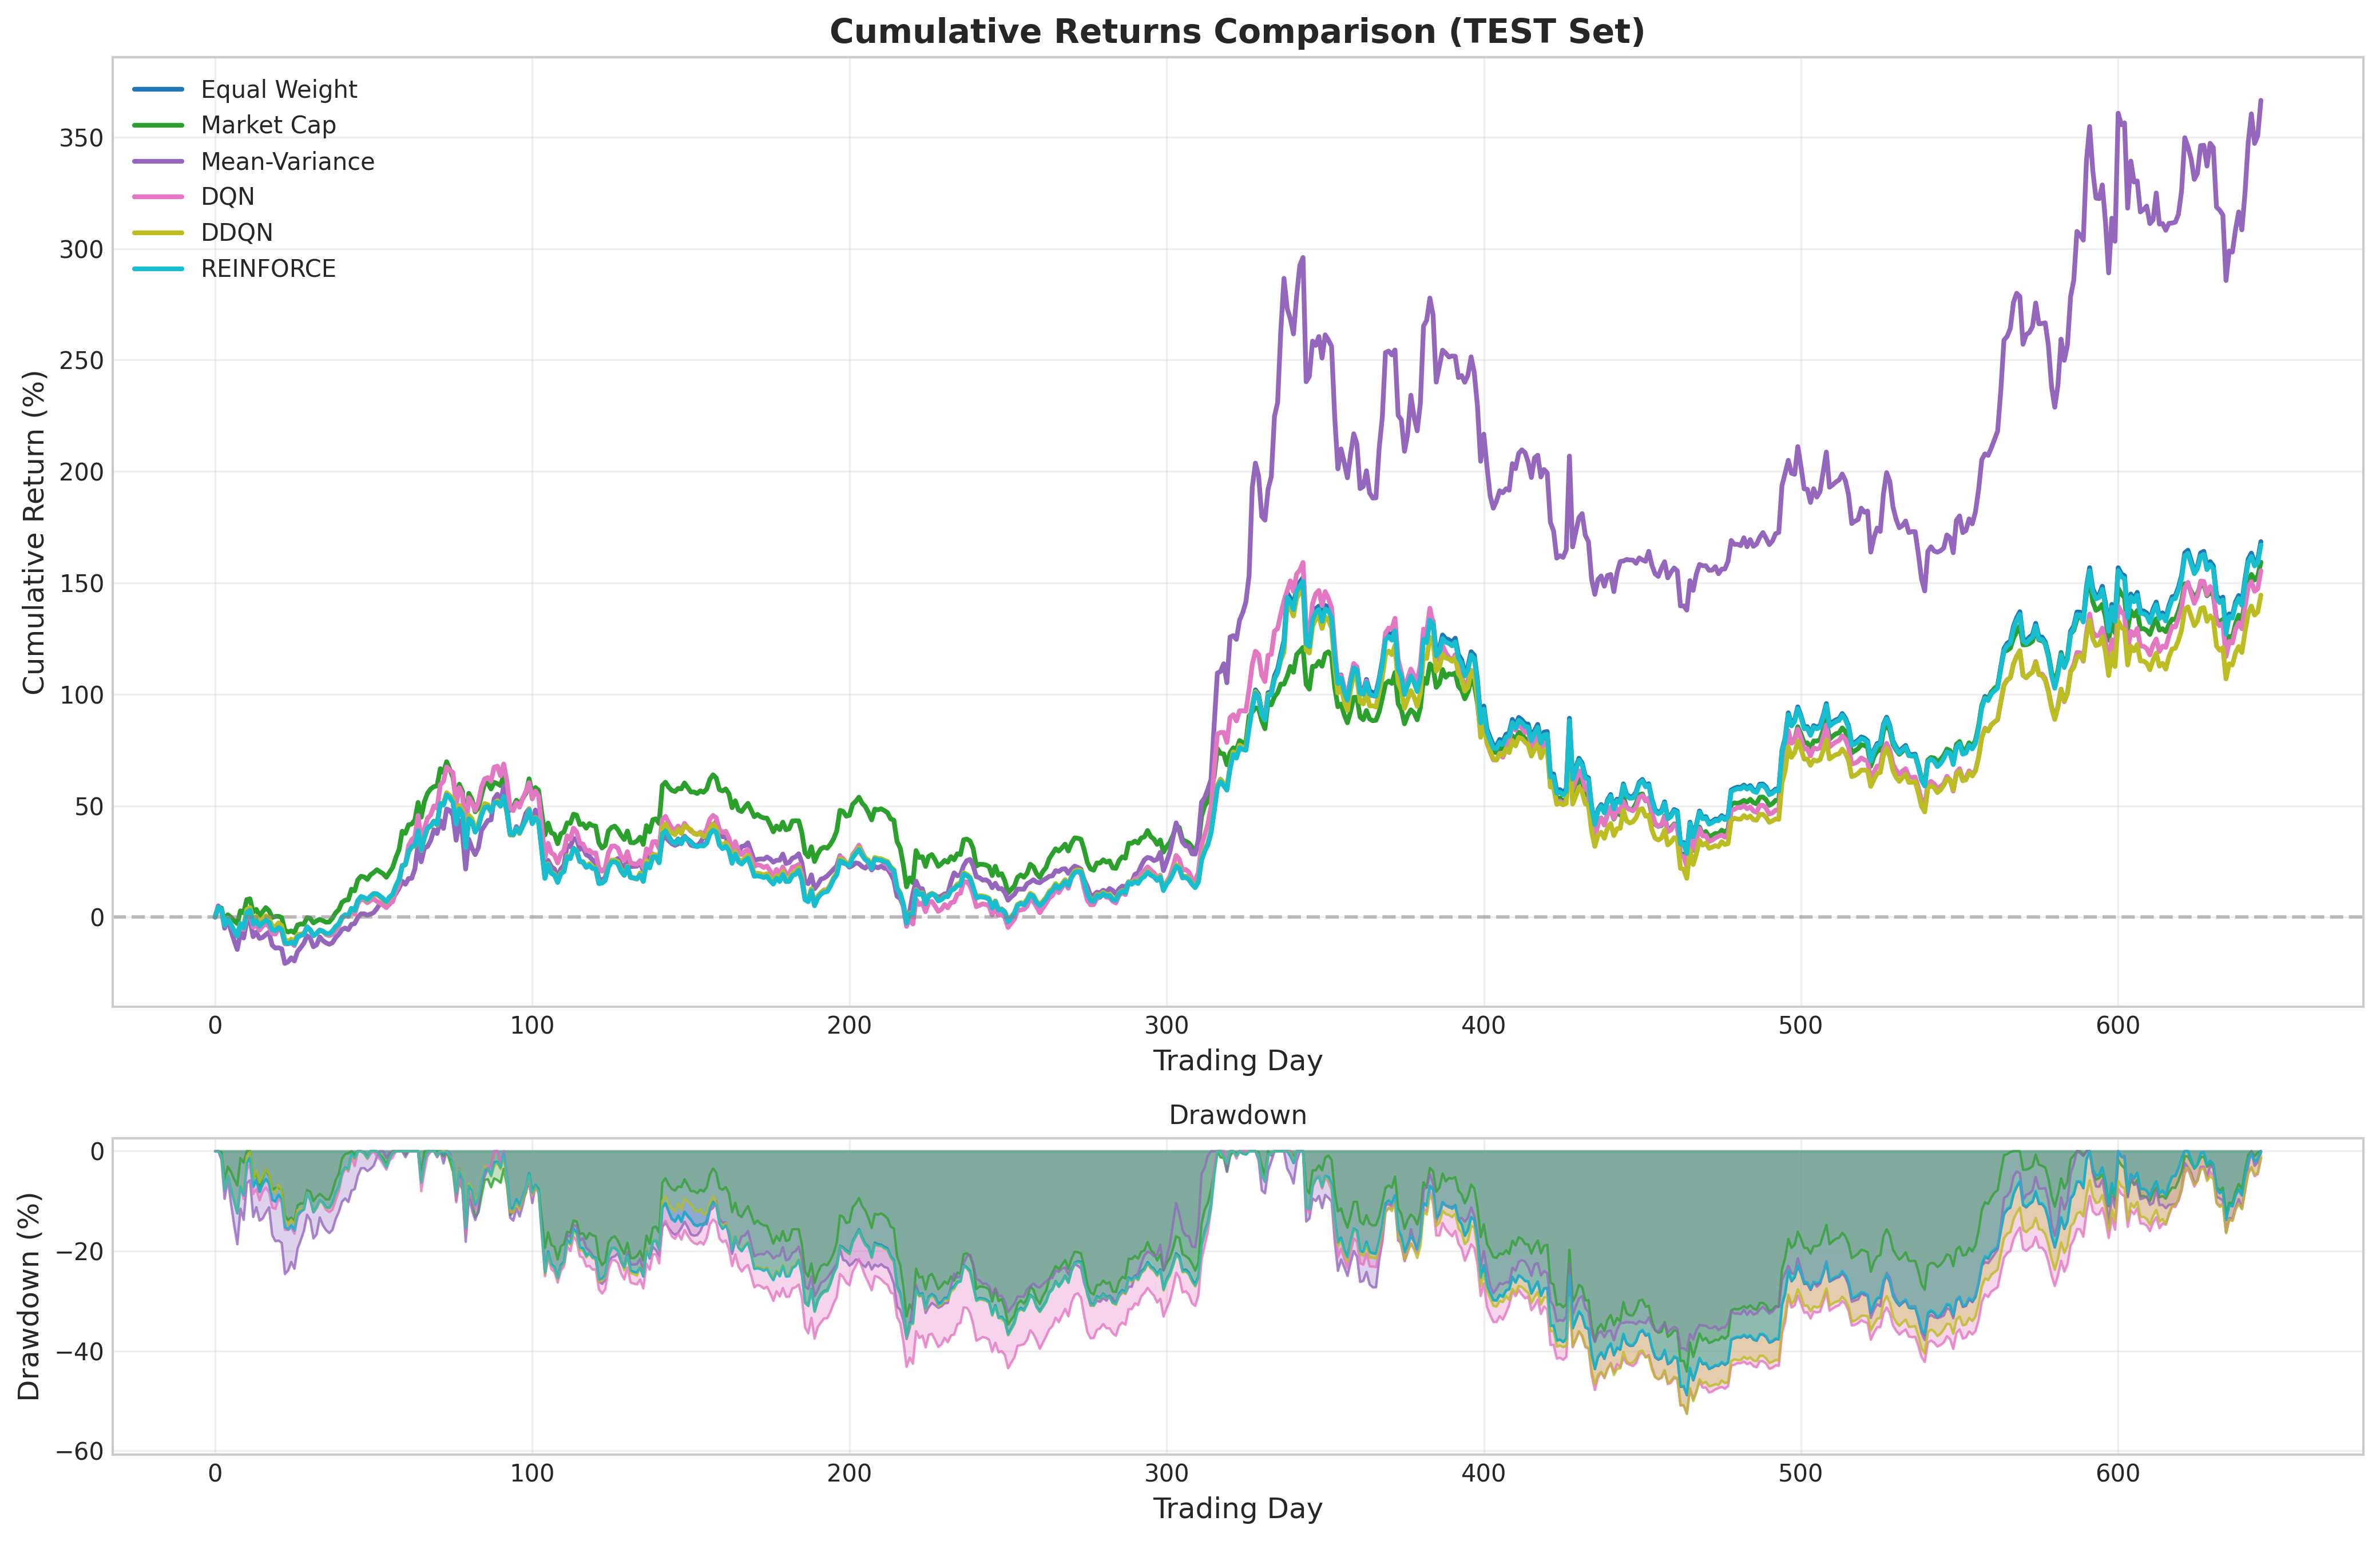
\includegraphics[width=\textwidth]{figures/cumulative_returns.png}
    \caption{Cumulative returns over the test period (January 2024 -- October 2025). Mean-Variance optimization substantially outperforms all other strategies, achieving 366\% cumulative return. The three RL agents (DQN, DDQN, REINFORCE) perform comparably to the Equal Weight baseline.}
    \label{fig:cumulative_returns}
\end{figure}

% Drawdown figure
\begin{figure}[htbp]
    \centering
    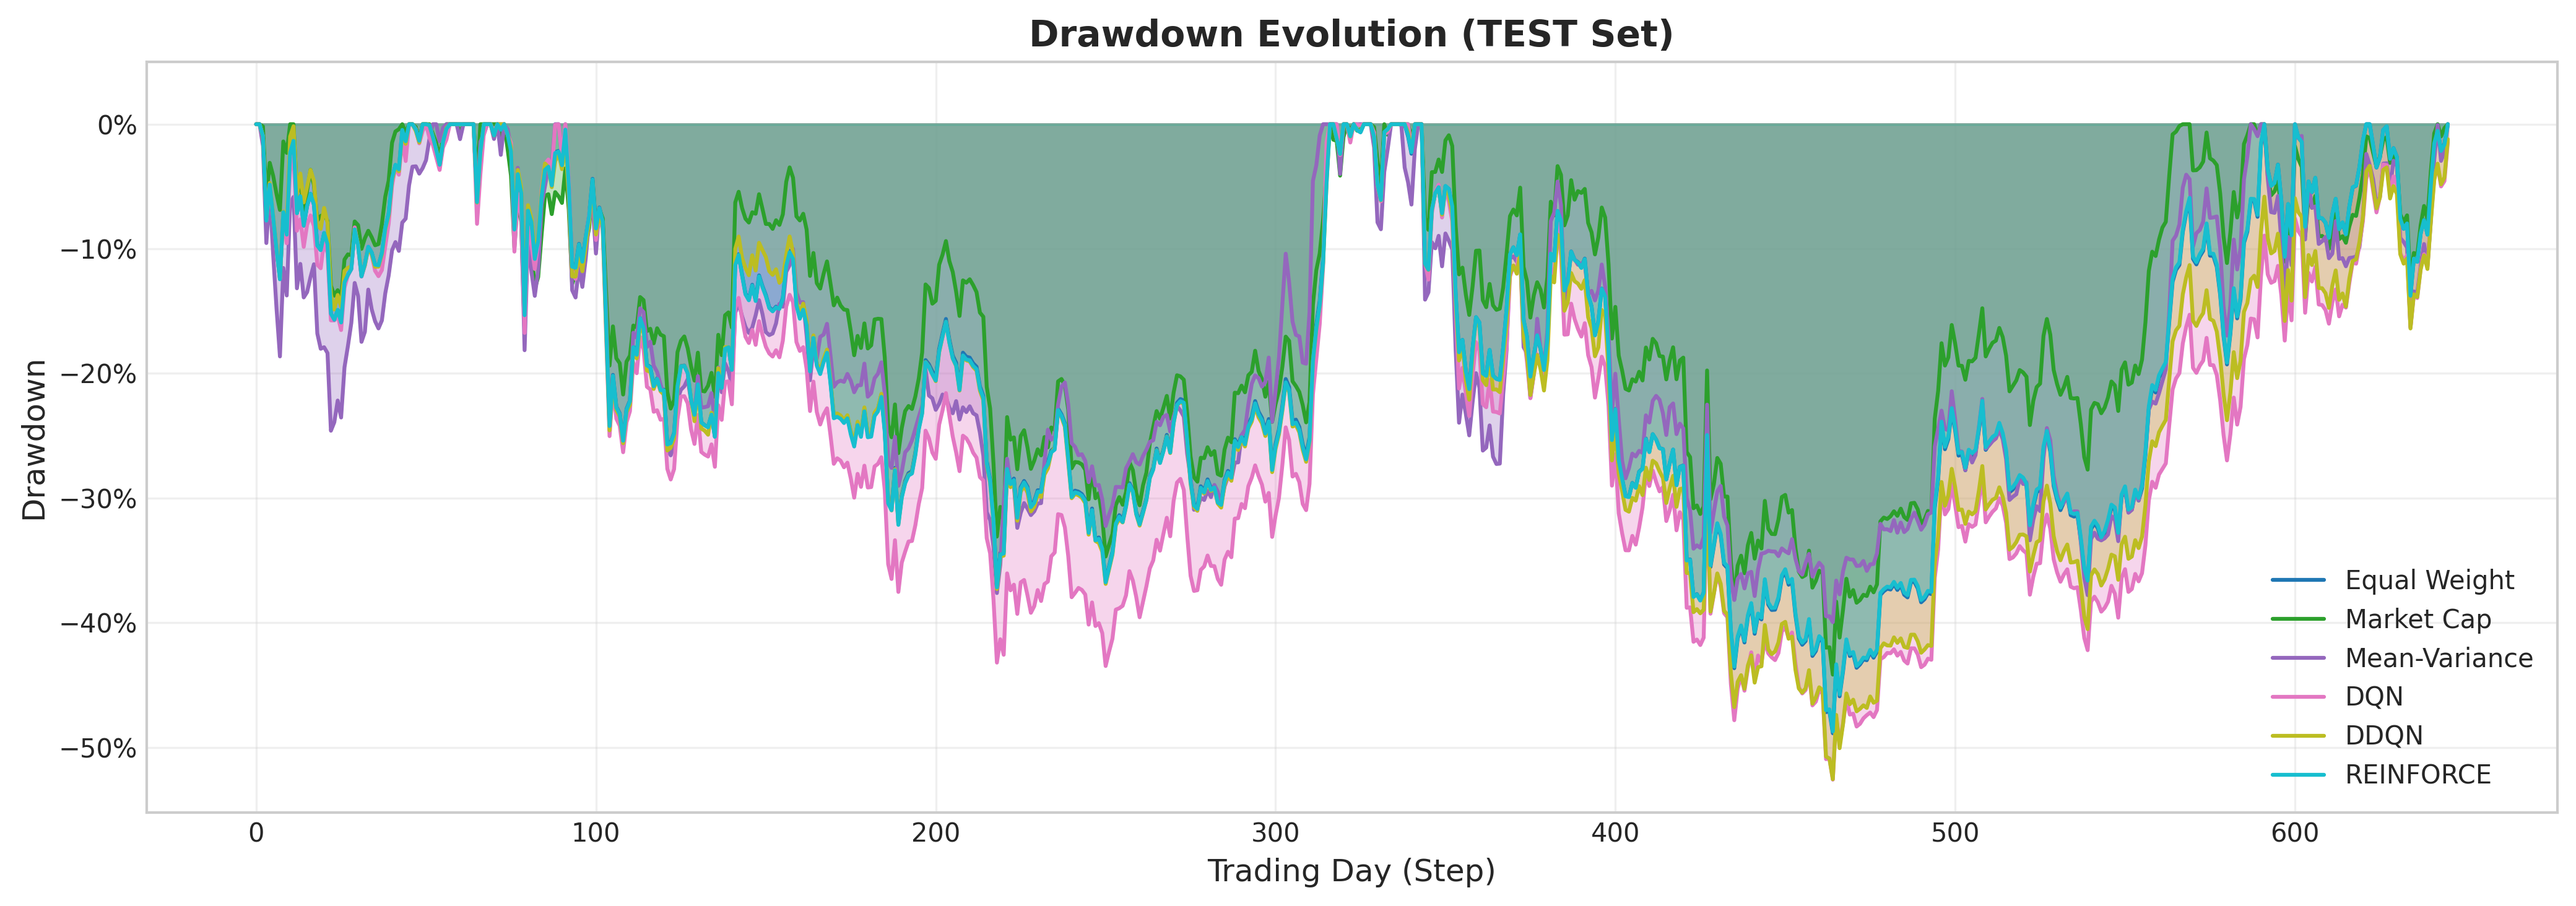
\includegraphics[width=\textwidth]{figures/drawdown.png}
    \caption{Drawdown analysis over the test period. Despite achieving the highest returns, Mean-Variance maintains the lowest maximum drawdown (39.96\%). The value-based RL agents (DQN, DDQN) experience the deepest drawdowns ($>$52\%).}
    \label{fig:drawdown}
\end{figure}

% Rolling Sharpe figure
\begin{figure}[htbp]
    \centering
    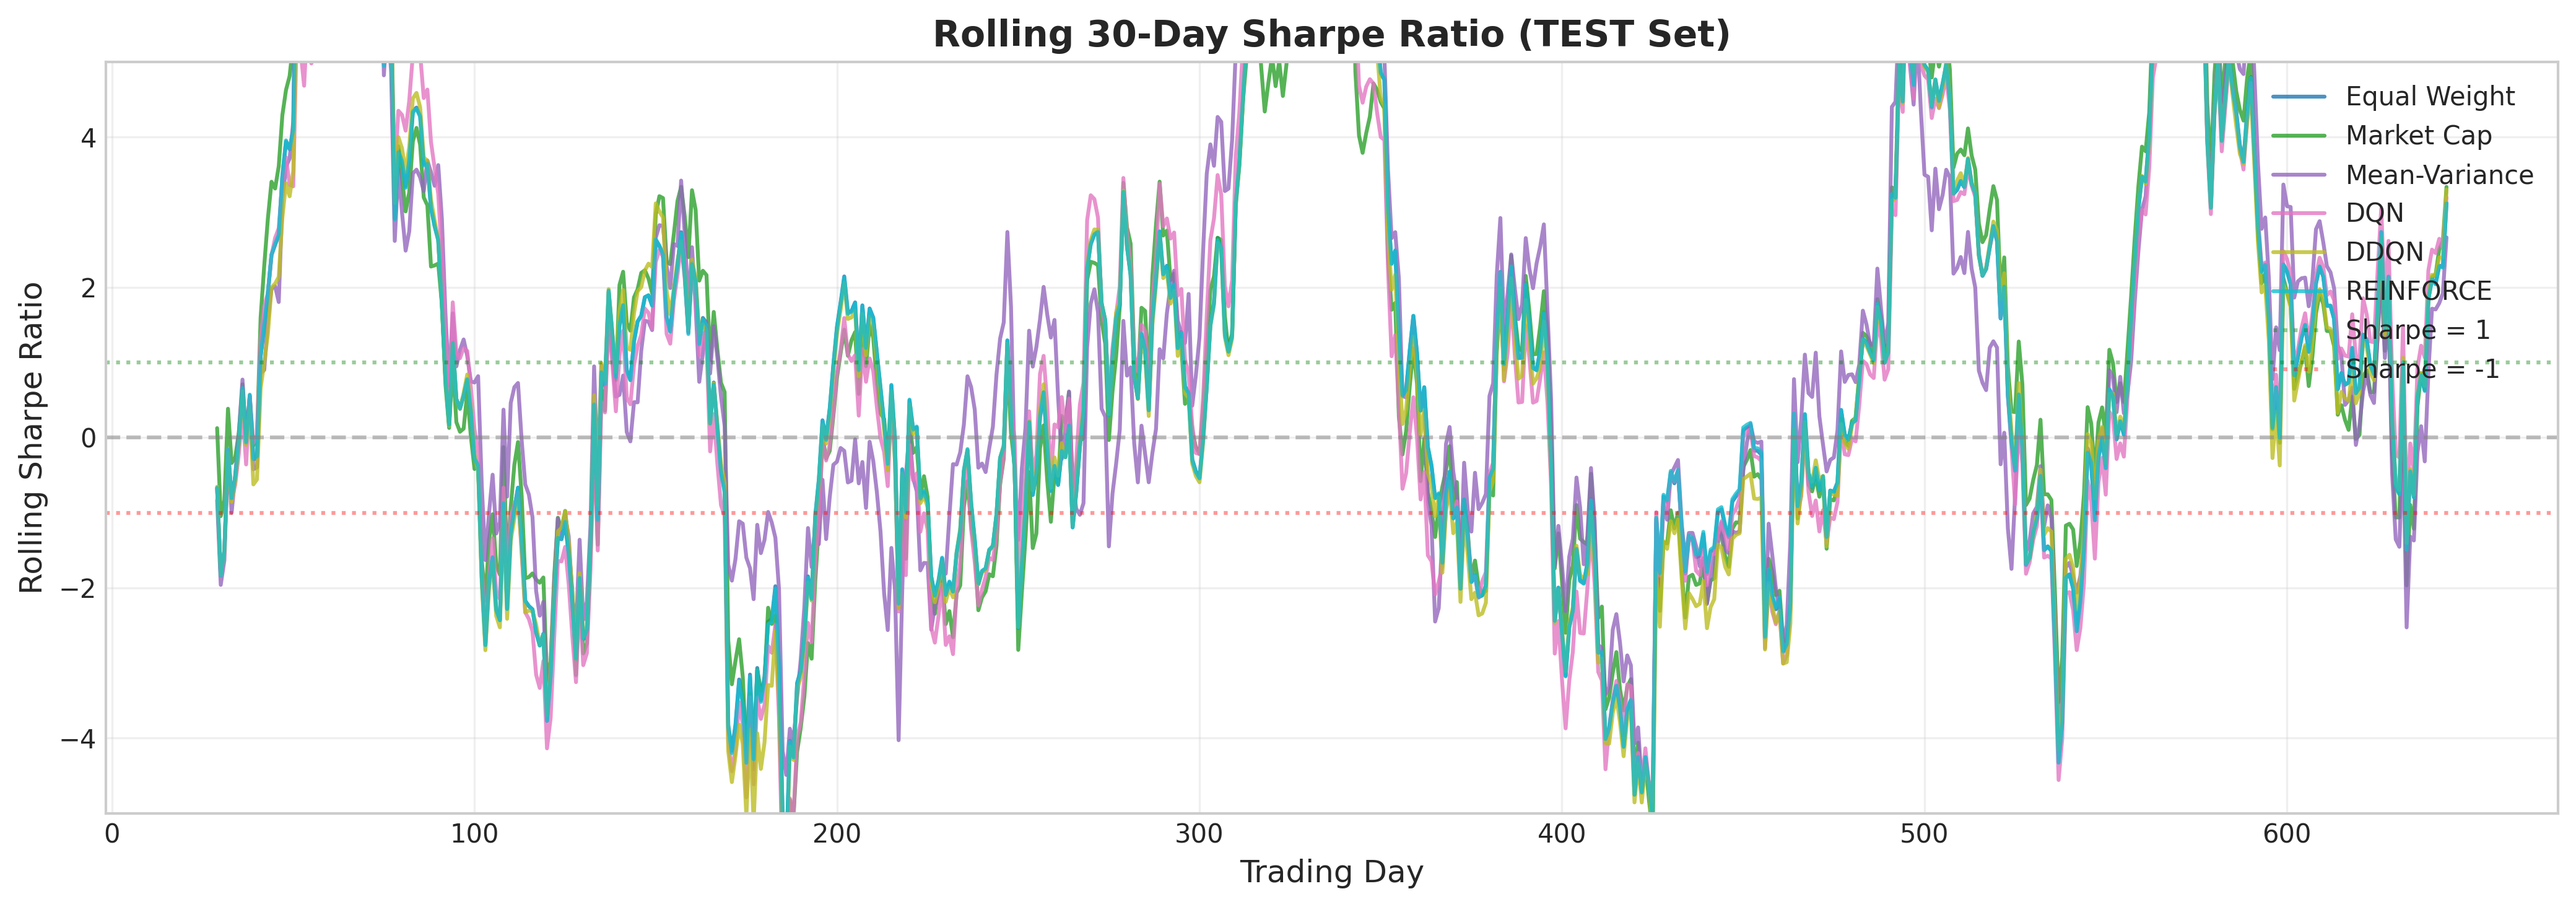
\includegraphics[width=\textwidth]{figures/rolling_sharpe.png}
    \caption{Rolling 60-day Sharpe ratio over the test period. Mean-Variance consistently maintains the highest risk-adjusted performance. All strategies show significant Sharpe ratio variation across different market regimes.}
    \label{fig:rolling_sharpe}
\end{figure}

% Allocation comparison figure
\begin{figure}[htbp]
    \centering
    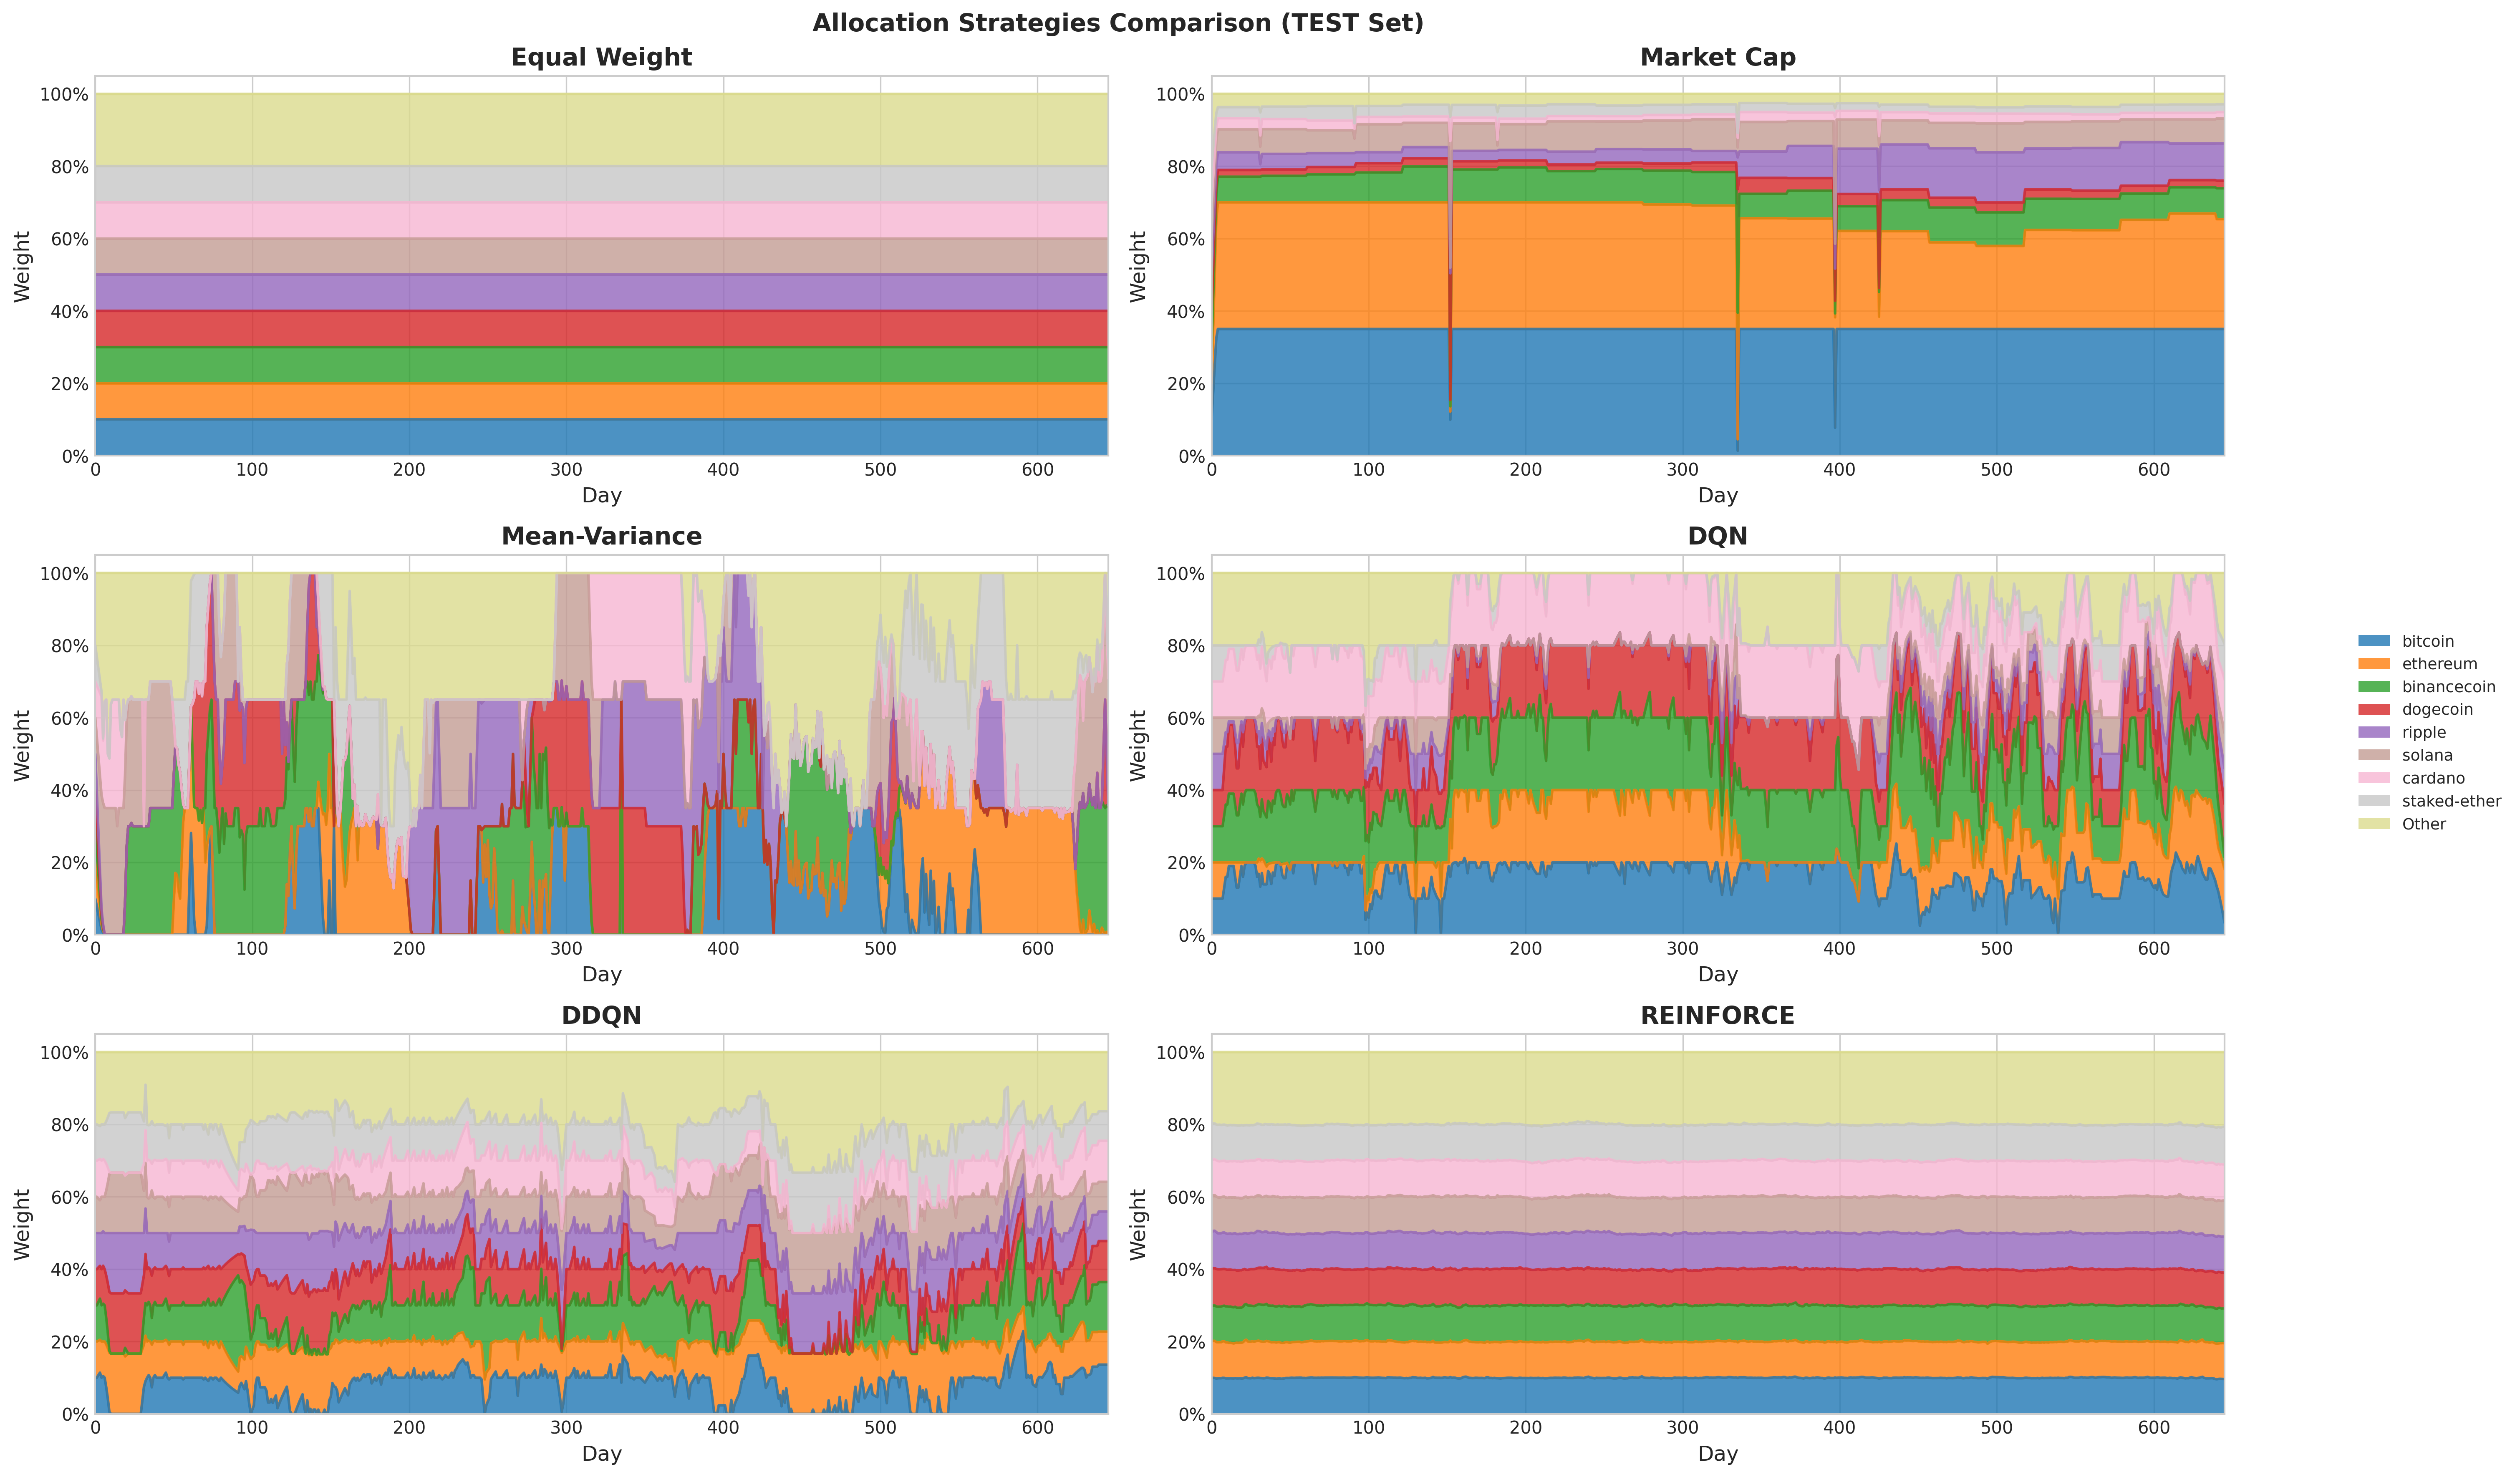
\includegraphics[width=\textwidth]{figures/allocation_comparison.png}
    \caption{Portfolio allocation comparison across strategies over the test period. Mean-Variance exhibits dynamic reallocation with concentrated positions, while Equal Weight maintains uniform distribution. REINFORCE closely mirrors Equal Weight behavior with near-uniform allocations, whereas DQN shows more active rebalancing with concentrated positions in select assets.}
    \label{fig:allocation_comparison}
\end{figure}

\paragraph{Key Observations.} Mean-Variance achieved the highest returns among all strategies, more than double that of the next-best strategy (366.54\% vs.\ 168.50\%), while simultaneously maintaining the highest Sharpe ratio (1.640) and the lowest maximum drawdown (39.96\%). This suggests that during our test period, historical return and covariance estimates provided genuinely useful predictive signal for cryptocurrency markets---a finding that warrants further investigation given the efficient market hypothesis often assumed in academic finance.

Among the reinforcement learning agents, REINFORCE achieved performance nearly identical to the Equal Weight baseline (166.98\% vs.\ 168.50\% return, 1.212 vs.\ 1.217 Sharpe), suggesting the learned policy converged toward a passive, low-turnover strategy. The allocation comparison in \Cref{fig:allocation_comparison} confirms this interpretation: REINFORCE maintains near-uniform allocations virtually indistinguishable from Equal Weight, indicating the policy gradient learned to minimize transaction costs rather than exploit predictive signals in the observation space.

The value-based agents underperformed all baselines. Both DQN (155.47\%) and DDQN (144.50\%) achieved lower returns than Equal Weight, Market Cap, and Mean-Variance. Their elevated turnover rates (10.88\% and 8.39\% respectively) suggest that the delta-based action space, while intuitive, encouraged excessive rebalancing that transaction costs ultimately penalized. Moreover, contrary to expectations from the broader RL literature~\citep{vanHasselt2016ddqn}, Double DQN performed worse than standard DQN in this domain; the reduced Q-value overestimation did not translate to improved portfolio performance.

Examining the turnover-return relationship more broadly, lower-turnover strategies (Equal Weight: 0.25\%, REINFORCE: 0.82\%) achieved competitive returns, while high-turnover strategies incurred significant transaction costs. Mean-Variance stands as the notable exception where active rebalancing generated substantial value, achieving 13.50\% daily turnover alongside superior risk-adjusted returns. The allocation dynamics in \Cref{fig:allocation_comparison} reveal that Mean-Variance dynamically shifts between concentrated and diversified positions based on rolling covariance estimates, while DQN frequently concentrates positions in select assets before rapidly rebalancing, explaining its high turnover without commensurate performance improvement.

% ============================================================
% DISCUSSION
% ============================================================

\section{Discussion}
\label{sec:discussion}

The results of our comparative evaluation contrast with positive results reported in prior reinforcement learning portfolio management studies. Mean-Variance optimization achieved 366\% cumulative return over the test period, more than double the next-best strategy, and outperformed all three RL agents on both absolute and risk-adjusted metrics. This section interprets these findings, situates them within the broader literature, acknowledges limitations, and identifies directions for future research.

% ------------------------------------------------------------
\subsection{Interpreting Mean-Variance Dominance}
\label{sec:mvo_analysis}
% ------------------------------------------------------------

The strong performance of Mean-Variance optimization admits several complementary explanations rooted in both market conditions and algorithmic characteristics. The test period spanning January 2024 through October 2025 coincided with a sustained cryptocurrency bull market following the prolonged bear market of 2022--2023. In trending market regimes, momentum signals embedded in rolling return estimates can carry predictive information, as recent winners tend to continue outperforming in the short term \cite{jegadeesh1993momentum}. The 60-day estimation window employed by our MVO baseline appears to have captured these momentum dynamics effectively, enabling the optimizer to concentrate allocations in assets with strong recent performance.

Beyond favorable market conditions, Mean-Variance optimization enjoys substantial sample efficiency advantages over reinforcement learning approaches. Where our RL agents required hundreds to thousands of training episodes to learn allocation policies through trial-and-error interaction, MVO directly estimates the sufficient statistics---expected returns and covariances---from historical data and solves a closed-form optimization problem. This estimation-based approach uses available data efficiently, whereas model-free RL must rediscover these statistical relationships through gradient descent on noisy reward signals. The Ledoit-Wolf shrinkage estimator~\citep{ledoit2004honey} further enhances MVO's robustness by addressing the instability of sample covariance matrices in high-dimensional settings \cite{ledoit2004honey}, regularizing estimates toward a structured target and reducing sensitivity to outliers.

We caution, however, that MVO's dominance may not generalize beyond the specific market conditions of our test period. Classical portfolio theory assumes stationary return distributions, an assumption violated in cryptocurrency markets characterized by regime shifts, bubble dynamics, and structural breaks \cite{james2022correlations}. In mean-reverting or highly volatile regimes where historical estimates lose predictive validity, the comparative advantage of MVO would likely diminish. The strong performance observed here should be interpreted as evidence that simple estimation-based methods remain competitive baselines rather than as a general indictment of learning-based approaches.

% ------------------------------------------------------------
\subsection{Explaining Reinforcement Learning Agent Behavior}
\label{sec:rl_analysis}
% ------------------------------------------------------------

The behavior of our reinforcement learning agents reveals instructive patterns about the challenges of applying deep RL to portfolio optimization. REINFORCE achieved performance nearly identical to the Equal Weight baseline (166.98\% vs.\ 168.50\% return), with portfolio allocations that converged to near-uniform distributions across tradable assets. This convergence suggests that the policy gradient learned to minimize transaction costs rather than exploit predictive signals in the observation space. Given the reward structure penalizing turnover at 0.1\% per unit rebalancing, a risk-averse policy that maintains stable allocations and avoids trading costs represents a local optimum that gradient descent may struggle to escape. This interpretation aligns with the theoretical analysis of~\citet{demiguel2009optimal}, who demonstrated that when estimation error dominates, naive diversification can outperform sophisticated optimization by avoiding costly mistakes.

The value-based agents underperformed all baselines. Both DQN (155.47\%) and DDQN (144.50\%) achieved lower returns than the three baseline strategies despite systematic hyperparameter optimization. Their elevated turnover rates of 10.88\% and 8.39\% respectively suggest that the delta-based action space, while intuitive for human interpretation, may have encouraged excessive rebalancing. Each action in our 70-action catalog applies a discrete portfolio adjustment, and the Q-network must learn which adjustments are profitable in which contexts---a challenging credit assignment problem when rewards are noisy and delayed. The observation that DDQN performed worse than standard DQN, contrary to expectations from the broader RL literature~\citep{vanHasselt2016ddqn}, indicates that reduced Q-value overestimation may have produced overly conservative policies in this domain, where some degree of optimism could encourage beneficial exploration.

Sample complexity poses a significant challenge for value-based methods in our setting. The canonical state representation spans 8,917 dimensions before projection, and the training budget of 400--500 episodes provides limited coverage of the state-action space. Prior work applying DQN to portfolio management~\citep{jiang2016drlt, lucarelli2020dqlcrypto} employed smaller asset universes and shorter lookback windows, reducing dimensionality and potentially easing the learning problem. Scaling deep RL to larger, more realistic portfolio settings may require architectural innovations such as attention mechanisms for cross-asset reasoning or hierarchical policies that separate regime detection from allocation decisions.

% ------------------------------------------------------------
\subsection{Comparison with Prior Work}
\label{sec:comparison_prior}
% ------------------------------------------------------------

Our findings contrast with several influential papers reporting strong RL outperformance in portfolio management. \citet{jiang2017eIIE} demonstrated that their EIIE architecture substantially outperformed baselines on cryptocurrency data from 2015--2017, a period characterized by the initial Bitcoin bull run and the emergence of altcoin markets. \citet{ye2020sarl} achieved similar success with state-augmented RL on Chinese equity markets. However, direct comparison is complicated by significant methodological differences: these studies employed smaller asset universes (12 assets vs.\ our 37), shorter evaluation periods, and in some cases did not impose realistic transaction cost structures.

The divergence between our results and prior claims admits several interpretations. First, market regime matters profoundly---the cryptocurrency landscape of 2024--2025 differs substantially from 2015--2017 in terms of market maturity, institutional participation, and correlation structure. Strategies that exploited inefficiencies in nascent markets may not transfer to more efficient conditions. Second, publication bias likely inflates reported RL performance, as negative results are systematically underrepresented in the literature. Our regime-diverse validation protocol and extended out-of-sample test period impose stricter evaluation standards than typical in this literature. Third, the fully-invested constraint in our formulation prevents agents from avoiding exposure during drawdowns, whereas some prior work permitted cash allocations that could trivially improve risk-adjusted metrics.

% ------------------------------------------------------------
\subsection{Limitations}
\label{sec:limitations}
% ------------------------------------------------------------

Several limitations temper the conclusions that can be drawn from this study. Most significantly, our test period represents a single market regime---a post-bear-market recovery transitioning into a bull market. Results from this favorable environment may not generalize to sustained bear markets, high-volatility crash periods, or prolonged sideways consolidation. A comprehensive evaluation would require testing across multiple complete market cycles, which the relatively short history of liquid cryptocurrency markets does not yet permit.

Our transaction cost model, while more realistic than many prior studies, remains simplified. The fixed 0.1\% cost per unit turnover ignores slippage, market impact, and the spread variation that characterizes cryptocurrency exchanges. Large rebalancing trades in less liquid assets would incur substantially higher implicit costs than our model assumes, potentially favoring concentrated positions in major assets. Additionally, our agents were frozen after training and evaluated without online adaptation. Continual learning approaches that update policies as market conditions evolve could narrow the gap with estimation-based methods that naturally incorporate recent data.

The hyperparameter search, while systematic, operated under computational constraints. Fifty Optuna trials may not have discovered optimal configurations for agents with high-dimensional hyperparameter spaces, and the episode budgets allocated for production training may have been insufficient for convergence, particularly for the value-based methods struggling with sample complexity. Finally, while Mean-Variance optimization substantially outperformed RL agents, it benefits from a form of hindsight through its rolling estimation window---returns observed after portfolio formation but within the estimation window for subsequent days implicitly inform allocations, a subtle advantage not available to RL agents trained on strictly historical data.

% ------------------------------------------------------------
\subsection{Implications and Future Directions}
\label{sec:future}
% ------------------------------------------------------------

Our findings carry implications for both practitioners and researchers working at the intersection of reinforcement learning and quantitative finance. For practitioners, the results underscore the importance of including simple baselines in any evaluation of learning-based portfolio strategies. The strong performance of Mean-Variance optimization---a technique dating to the 1950s---relative to deep RL architectures indicates that more complex methods do not automatically outperform classical approaches in financial domains. Any deployment of RL-based allocation systems should demonstrate clear outperformance against classical alternatives under realistic transaction cost assumptions and across diverse market conditions.

For the research community, our results highlight several promising directions for advancing RL portfolio management. The sample complexity challenges faced by our value-based agents suggest that architectural innovations enabling more efficient learning deserve priority. Transformer architectures with cross-asset attention mechanisms could enable agents to reason about correlation structure without explicit estimation, potentially combining the strengths of MVO and deep learning. Hierarchical reinforcement learning offers another avenue, decomposing the allocation problem into regime detection at a slow timescale and tactical positioning at a fast timescale. Such decomposition could improve credit assignment and enable transfer learning across market regimes. Finally, online and continual learning approaches that adapt policies to evolving market conditions could address the non-stationarity that fundamentally limits offline-trained agents. The gap between research benchmarks and practical deployment remains substantial, and closing it will require sustained attention to evaluation methodology, computational efficiency, and robustness to distribution shift.

% ============================================================
% CONCLUSION
% ============================================================

\section{Conclusion}
\label{sec:conclusion}

This paper investigated the application of deep reinforcement learning to cryptocurrency portfolio management, comparing four RL agents against classical baselines on a rigorous 646-day out-of-sample test. Our evaluation employed a realistic environment with monthly universe reconstitution, transaction costs, and turnover constraints, providing a more stringent benchmark than typical in this literature.

The central finding is that algorithmic paradigm and inference-time behavior both matter: DDQN's value-based approach with discrete delta actions outperformed all methods except MVO, while REINFORCE's continuous Dirichlet policy achieved competitive performance (167\% with baseline) when using deterministic evaluation that outputs the distribution mean rather than sampling. This demonstrates that policy gradient agents can learn meaningful allocation preferences, but realizing this potential requires appropriate inference-time behavior. Mean-Variance optimization's dominance (366\% return) further demonstrates that classical estimation-based methods remain formidable competitors when market conditions favor momentum-based signals.

Our methodological contributions---the variable-universe environment with canonical padding, delta-based discrete action space, and frozen dataset export---address practical challenges that prior work largely ignored and enable exact reproduction of our experiments.

Several directions merit future investigation: deterministic policy gradient methods (DDPG, TD3) that provide a natural middle ground between discrete and sampled continuous actions; transformer architectures with cross-asset attention for implicit correlation modeling; extended evaluation across bear markets and crash periods; investigation of stochastic versus deterministic deployment tradeoffs; and online learning approaches that adapt to evolving market dynamics. Our results suggest that the gap between research benchmarks and practical deployment is narrower than sometimes claimed---careful implementation of established RL algorithms can yield portfolio strategies that outperform passive investment approaches.


% ------------------------------------------------------------
% BIBLIOGRAPHY
% ------------------------------------------------------------
\bibliographystyle{plainnat}
\bibliography{bibliography}

% ------------------------------------------------------------
% APPENDIX (optional)
% ------------------------------------------------------------
\appendix
% ============================================================
% APPENDIX
% ============================================================

\section{Hyperparameter Settings}
\label{app:hyperparameters}

% DQN Hyperparameters
\begin{table}[htbp]
\centering
\caption{DQN and DDQN hyperparameters.}
\label{tab:dqn_hyperparams}
\begin{tabular}{lcc}
\toprule
\textbf{Hyperparameter} & \textbf{DQN} & \textbf{DDQN} \\
\midrule
Learning rate & & \\
Batch size & & \\
Replay buffer size & & \\
Target update frequency & & \\
Discount factor ($\gamma$) & & \\
Epsilon start & & \\
Epsilon end & & \\
Epsilon decay & & \\
Hidden dimensions & & \\
\bottomrule
\end{tabular}
\end{table}

% REINFORCE Hyperparameters
\begin{table}[htbp]
\centering
\caption{REINFORCE hyperparameters.}
\label{tab:reinforce_hyperparams}
\begin{tabular}{lc}
\toprule
\textbf{Hyperparameter} & \textbf{Value} \\
\midrule
Learning rate & \\
GRU hidden size & \\
Number of GRU layers & \\
Dropout & \\
Discount factor ($\gamma$) & \\
Entropy coefficient & \\
\bottomrule
\end{tabular}
\end{table}

% ------------------------------------------------------------

\section{Action Catalog}
\label{app:action_catalog}

% TODO: Full list of 70 delta-based actions
% Table or enumeration of action categories

% ------------------------------------------------------------

\section{Additional Figures}
\label{app:additional_figures}

% TODO: Include additional visualizations
% - Portfolio weight evolution
% - Training curves
% - Drawdown analysis


\end{document}
